\begin{Problem}{Acesrc and Cube Hypernet}{2}

Given a 3-dimensional cube, if we cut some edges, the surface of the cube can be unfolded into 2-dimensional space. Such flat shape is called a \textit{cube net}. There are 11 essentially different cube nets, listed below.

\begin{figure}[htb]
\centering
\includegraphics[width=12cm]{nets.jpg}
\caption{The 11 essentially different cube nets.}
\end{figure}

In this problem, we consider a generalization of the cube net, called \textit{cube hypernet}. For each face of a cube, we divide it into $k \times k$ small square cells. If we cut some edges of these small cells, the surface of the cube can be unfolded into 2-dimensional space, then the resulting flat shape is a cube hypernet. Clearly, cube nets are just a special type of cube hypernets where $k = 1$. The following picture illustrates a cube hypernet and explains how it is formed.

\begin{figure}[htb]
\centering

\tikzset{every picture/.style={line width=0.75pt}} %set default line width to 0.75pt        

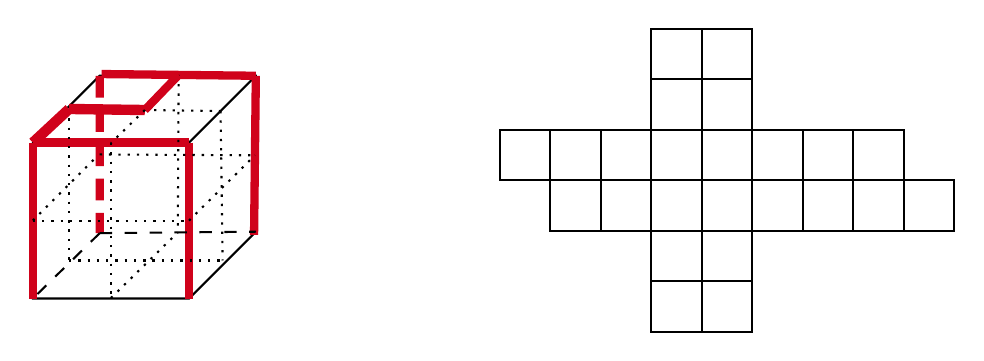
\begin{tikzpicture}[x=0.75pt,y=0.75pt,yscale=-1,xscale=1]
%uncomment if require: \path (0,300); %set diagram left start at 0, and has height of 300

%Shape: Cube [id:dp5713421173433544] 
\draw   (92,119.87) -- (124.2,87.67) -- (199.43,87.67) -- (199.43,162.8) -- (167.23,195) -- (92,195) -- cycle ; \draw   (199.43,87.67) -- (167.23,119.87) -- (92,119.87) ; \draw   (167.23,119.87) -- (167.23,195) ;
%Straight Lines [id:da42563945957545957] 
\draw [color={rgb, 255:red, 208; green, 2; blue, 27 }  ,draw opacity=1 ][line width=3]    (92,119.87) -- (92,195) ;


%Straight Lines [id:da11360839227996866] 
\draw [color={rgb, 255:red, 208; green, 2; blue, 27 }  ,draw opacity=1 ][line width=3]    (92,119.87) -- (167.23,119.87) ;


%Straight Lines [id:da5837990090607357] 
\draw [color={rgb, 255:red, 208; green, 2; blue, 27 }  ,draw opacity=1 ][line width=3]  [dash pattern={on 7.88pt off 4.5pt}]  (124.2,87.67) -- (124.22,163.49) ;


%Straight Lines [id:da3949397955529803] 
\draw [color={rgb, 255:red, 208; green, 2; blue, 27 }  ,draw opacity=1 ][line width=3]    (125.08,86.84) -- (199.43,87.67) ;


%Straight Lines [id:da4851398910346689] 
\draw [color={rgb, 255:red, 208; green, 2; blue, 27 }  ,draw opacity=1 ][line width=3]    (167.23,119.87) -- (167.23,195) ;


%Straight Lines [id:da7311203923035952] 
\draw [color={rgb, 255:red, 208; green, 2; blue, 27 }  ,draw opacity=1 ][line width=3]    (199.43,87.67) -- (198.57,164.32) ;


%Straight Lines [id:da7022479459425415] 
\draw  [dash pattern={on 4.5pt off 4.5pt}]  (124.22,163.49) -- (199.43,162.8) ;


%Straight Lines [id:da7189806870957662] 
\draw  [dash pattern={on 4.5pt off 4.5pt}]  (124.22,163.49) -- (92,195) ;


%Straight Lines [id:da9178045604326999] 
\draw [color={rgb, 255:red, 0; green, 0; blue, 0 }  ,draw opacity=1 ] [dash pattern={on 0.84pt off 2.51pt}]  (145.93,104.17) -- (182.43,104.67) ;


%Straight Lines [id:da04301172838480838] 
\draw [color={rgb, 255:red, 0; green, 0; blue, 0 }  ,draw opacity=1 ] [dash pattern={on 0.84pt off 2.51pt}]  (92,157.43) -- (167.23,157.43) ;


%Straight Lines [id:da9145997008953277] 
\draw [color={rgb, 255:red, 0; green, 0; blue, 0 }  ,draw opacity=1 ] [dash pattern={on 0.84pt off 2.51pt}]  (129.61,120.12) -- (129.61,194.75) ;


%Straight Lines [id:da9400584505703131] 
\draw  [dash pattern={on 0.84pt off 2.51pt}]  (109.43,103.67) -- (109.43,176.67) ;


%Straight Lines [id:da4339187022384017] 
\draw  [dash pattern={on 0.84pt off 2.51pt}]  (92,157.43) -- (123.43,126.01) ;


%Straight Lines [id:da12326295357742123] 
\draw  [dash pattern={on 0.84pt off 2.51pt}]  (109.43,176.67) -- (183.43,176.67) ;


%Straight Lines [id:da859413357855844] 
\draw  [dash pattern={on 0.84pt off 2.51pt}]  (129.61,194.75) -- (161.82,163.15) ;


%Straight Lines [id:da22416829329673393] 
\draw  [dash pattern={on 0.84pt off 2.51pt}]  (162.25,87.25) -- (161.82,163.15) ;


%Straight Lines [id:da5602089262552088] 
\draw  [dash pattern={on 0.84pt off 2.51pt}]  (124.21,125.58) -- (199,125.99) ;


%Straight Lines [id:da9523299030375125] 
\draw  [dash pattern={on 0.84pt off 2.51pt}]  (167.23,157.43) -- (199,125.99) ;


%Straight Lines [id:da5451371565037118] 
\draw  [dash pattern={on 0.84pt off 2.51pt}]  (182.43,104.67) -- (183.43,176.67) ;


%Shape: Square [id:dp7591135470696151] 
\draw   (390,65) -- (414.33,65) -- (414.33,89.33) -- (390,89.33) -- cycle ;
%Shape: Square [id:dp917157522376586] 
\draw   (390,89.33) -- (414.33,89.33) -- (414.33,113.67) -- (390,113.67) -- cycle ;
%Shape: Square [id:dp6066190461876488] 
\draw   (414.33,65) -- (438.67,65) -- (438.67,89.33) -- (414.33,89.33) -- cycle ;
%Shape: Square [id:dp23412140295087092] 
\draw   (414.33,89.33) -- (438.67,89.33) -- (438.67,113.67) -- (414.33,113.67) -- cycle ;
%Shape: Square [id:dp39521998722950746] 
\draw   (390,113.67) -- (414.33,113.67) -- (414.33,138) -- (390,138) -- cycle ;
%Shape: Square [id:dp7597028280692992] 
\draw   (390,138) -- (414.33,138) -- (414.33,162.33) -- (390,162.33) -- cycle ;
%Shape: Square [id:dp9032016100512299] 
\draw   (414.33,113.67) -- (438.67,113.67) -- (438.67,138) -- (414.33,138) -- cycle ;
%Shape: Square [id:dp9862136660298677] 
\draw   (414.33,138) -- (438.67,138) -- (438.67,162.33) -- (414.33,162.33) -- cycle ;
%Shape: Square [id:dp2105696458351256] 
\draw   (390,162.33) -- (414.33,162.33) -- (414.33,186.67) -- (390,186.67) -- cycle ;
%Shape: Square [id:dp38203525928531445] 
\draw   (414.33,162.33) -- (438.67,162.33) -- (438.67,186.67) -- (414.33,186.67) -- cycle ;
%Shape: Square [id:dp07452681855437948] 
\draw   (390,186.67) -- (414.33,186.67) -- (414.33,211) -- (390,211) -- cycle ;
%Shape: Square [id:dp46685422276231514] 
\draw   (414.33,186.67) -- (438.67,186.67) -- (438.67,211) -- (414.33,211) -- cycle ;
%Shape: Square [id:dp1815129932944446] 
\draw   (438.67,113.67) -- (463,113.67) -- (463,138) -- (438.67,138) -- cycle ;
%Shape: Square [id:dp8928307047272608] 
\draw   (438.67,138) -- (463,138) -- (463,162.33) -- (438.67,162.33) -- cycle ;
%Shape: Square [id:dp3917633232801916] 
\draw   (463,113.67) -- (487.34,113.67) -- (487.34,138) -- (463,138) -- cycle ;
%Shape: Square [id:dp4091908537319717] 
\draw   (463,138) -- (487.34,138) -- (487.34,162.33) -- (463,162.33) -- cycle ;
%Shape: Square [id:dp3525235222171257] 
\draw   (365.67,113.67) -- (390,113.67) -- (390,138) -- (365.67,138) -- cycle ;
%Shape: Square [id:dp5339668640142305] 
\draw   (365.67,138) -- (390,138) -- (390,162.33) -- (365.67,162.33) -- cycle ;
%Shape: Square [id:dp8907339502163012] 
\draw   (341.33,113.67) -- (365.67,113.67) -- (365.67,138) -- (341.33,138) -- cycle ;
%Shape: Square [id:dp4554401476147847] 
\draw   (341.33,138) -- (365.67,138) -- (365.67,162.33) -- (341.33,162.33) -- cycle ;
%Shape: Square [id:dp633196329874429] 
\draw   (317,113.67) -- (341.33,113.67) -- (341.33,138) -- (317,138) -- cycle ;
%Shape: Square [id:dp062935463038297] 
\draw   (511.67,138) -- (536,138) -- (536,162.33) -- (511.67,162.33) -- cycle ;
%Shape: Square [id:dp8856843680936886] 
\draw   (487.34,113.67) -- (511.67,113.67) -- (511.67,138) -- (487.34,138) -- cycle ;
%Shape: Square [id:dp514905839618633] 
\draw   (487.34,138) -- (511.67,138) -- (511.67,162.33) -- (487.34,162.33) -- cycle ;
%Straight Lines [id:da9682499505773039] 
\draw [color={rgb, 255:red, 208; green, 2; blue, 27 }  ,draw opacity=1 ][line width=3]    (145.93,104.17) -- (162.25,87.25) ;


%Straight Lines [id:da17272908888168392] 
\draw [color={rgb, 255:red, 208; green, 2; blue, 27 }  ,draw opacity=1 ][line width=3.75]    (109.43,103.67) -- (145.93,104.17) ;


%Straight Lines [id:da7081830858409768] 
\draw [color={rgb, 255:red, 208; green, 2; blue, 27 }  ,draw opacity=1 ][line width=3.75]    (109.43,103.67) -- (92,119.87) ;


%Straight Lines [id:da379429243876815] 
\draw  [dash pattern={on 0.84pt off 2.51pt}]  (145.93,104.17) -- (129.61,120.12) ;


\end{tikzpicture}
\caption{A cube hypernet.}
\end{figure}

Identifying cube nets is a relatively easy job, however, this might not be true for cube hypernets. Here comes the challenge. Given a flat shape composed of small squares, determine whether it is a cube hypernet.

\subsection*{Input}

The first line of the input is a single integer $T$ $(1 \leq T \leq 30)$, denoting the number of test cases. 

For each test case, the first line contains two integers $h, w$ $(1 \leq h, w \leq 100)$, denoting the height and width of the input region. For the remaining $h$ lines, each containing $w$ characters, either \texttt{'\#'} or \texttt{'.'}. The character \texttt{'\#'} means that the square is part of the shape, while the character \texttt{'.'} means that the square is not part of the shape.

It is guaranteed that the input shape is nonempty and connected in four directions, and there is no hole inside the shape, not even a hole 8-connected to the outside. Also, the sum of $h \times w$ over all test cases does not exceed 35000.

\subsection*{Output}

For each test case, output \texttt{yes} in a line if the input shape is cube hypernet, and \texttt{no} otherwise.

\exmpv{cube}

\end{Problem}
